\documentclass[11pt,a4paper]{article}

\usepackage[margin=1in]{geometry}
\usepackage{amsmath,amssymb,amsthm}
\usepackage{graphicx}
\usepackage{booktabs}
\usepackage{enumitem}
\usepackage{hyperref}
\usepackage{xcolor}
\usepackage{listings}
\usepackage{algorithm}
\usepackage{algorithmic}
\usepackage{tcolorbox}
\usepackage{fancyhdr}
\usepackage{multicol}
\usepackage{fontawesome5}

\tcbuselibrary{breakable,skins}

% Theorem environments
\theoremstyle{definition}
\newtheorem{definition}{Definition}[section]
\newtheorem{example}{Example}[section]
\newtheorem{remark}{Remark}[section]
\theoremstyle{plain}
\newtheorem{proposition}{Proposition}[section]

% Custom boxes
\newtcolorbox{keytakeaway}{colback=green!5!white,colframe=green!50!black,title={Key Takeaway},fonttitle=\bfseries,breakable}
\newtcolorbox{pitfall}{colback=red!5!white,colframe=red!60!black,title={Common Pitfall},fonttitle=\bfseries,breakable}
\newtcolorbox{production}{colback=blue!5!white,colframe=blue!50!black,title={Production Note},fonttitle=\bfseries,breakable}

% Code listings
\lstset{language=Python,basicstyle=\ttfamily\footnotesize,keywordstyle=\color{blue},commentstyle=\color{gray},stringstyle=\color{red},showstringspaces=false,breaklines=true,frame=single,numbers=left,numberstyle=\tiny\color{gray},backgroundcolor=\color{gray!10},xleftmargin=2em,framexleftmargin=1.5em}

% TikZ libraries for included figures
\usetikzlibrary{shapes,arrows,positioning,calc,patterns,decorations.pathreplacing,shadows,fit}

% Header/Footer
\pagestyle{fancy}
\fancyhf{}
\fancyhead[L]{\textsc{Information Retrieval}}
\fancyhead[R]{\textsc{Lecture 2: Sparse and Dense Indexing}}
\fancyfoot[C]{\thepage}

\title{\textbf{Lecture 2: Sparse and Dense Indexing}\\[0.5em]\Large Information Retrieval --- Lecture Notes}
\author{Avishek Anand\\\textit{Information Retrieval Course}}
\date{\today}
% Custom macros and TikZ styles
\usepackage{tikz}
\usetikzlibrary{positioning, shapes, arrows, shadows, fit, calc, decorations.pathreplacing}

% Semantic Colors - One meaning per color
\definecolor{irSparse}{HTML}{3498DB}   % Sparse/BM25: Blue
\definecolor{irDense}{HTML}{E67E22}    % Dense/Embeddings: Orange
\definecolor{irRerank}{HTML}{C0392B}   % Rerank/Cross-encoder: Red
\definecolor{irHybrid}{HTML}{2ECC71}   % Hybrid/Fusion: Green
\definecolor{irANN}{HTML}{9B59B6}      % ANN/Infra: Purple
\definecolor{irInfra}{HTML}{58595B}    % General Infra: Dark Gray
\definecolor{irMuted}{HTML}{D9D9D9}    % Faint Gray

% Base Styles - Consistent Diagram Grammar
\tikzset{
    irBoxBase/.style={
        rectangle, 
        draw, 
        rounded corners=2pt, 
        minimum height=0.8cm, 
        minimum width=2cm,
        font=\small\sffamily,
        align=center,
        drop shadow={opacity=0.15},
        inner sep=5pt
    },
    irDatabase/.style={
        cylinder, 
        draw, 
        shape border rotate=90, 
        aspect=0.25, 
        minimum height=1.2cm, 
        minimum width=1cm,
        fill=irMuted!20,
        draw=irInfra,
        font=\tiny\sffamily,
        align=center
    },
    % Semantic Variants
    sparse/.style={irBoxBase, fill=irSparse!10, draw=irSparse},
    dense/.style={irBoxBase, fill=irDense!10, draw=irDense},
    rerank/.style={irBoxBase, fill=irRerank!10, draw=irRerank},
    hybrid/.style={irBoxBase, fill=irHybrid!10, draw=irHybrid},
    ann/.style={irBoxBase, fill=irANN!10, draw=irANN},
    infra/.style={irBoxBase, fill=irInfra!10, draw=irInfra},
    % Legacy support / Utility
    muted/.style={irBoxBase, fill=irMuted!20, draw=irMuted!80!black, text=irMuted!50!black},
    ghost/.style={irBoxBase, fill=white, draw=irMuted!50, text=irMuted, dashed, drop shadow={opacity=0}},
    emph/.style={draw=irRerank, thick, drop shadow={shadow xshift=0mm, shadow yshift=0mm, fill=irRerank, opacity=0.3}},
    % Arrows
    irArrowBase/.style={->, thick, >=latex, draw=irInfra},
    irLabel/.style={
        font=\tiny\itshape, 
        text=irInfra, 
        align=center, 
        text width=2.5cm, 
        inner sep=3pt
    }
}


% =========================================================
% Stage Badge System
% =========================================================
% \irStage{StageName}
\newcommand{\irStage}[1]{%
    \begin{tikzpicture}[remember picture, overlay]
        \node[
            anchor=north east,
            fill=irInfra!10,
            text=irInfra,
            font=\tiny\bfseries,
            inner sep=3pt,
            rounded corners=1pt,
            yshift=-0.5cm,
            xshift=-0.5cm
        ] at (current page.north east) {#1};
    \end{tikzpicture}%
}

% =========================================================
% Math Highlighting
% =========================================================
% \mathhl[color]{content}
\newcommand{\mathhl}[2][irDense!30]{%
    \colorbox{#1}{$\displaystyle #2$}%
}

% =========================================================
% Math Vectors
% =========================================================
\newcommand{\vs}{\mathbf{s}}

% =========================================================
% Core Box Primitives
% =========================================================
% \IRBox[width]{id}{at}{title}{subtitle}{variant}
% Default width chosen for lecture slides; override when needed.
% \IRBox[width]{id}{at}{title}{subtitle}{variant}[extra options]
\DeclareDocumentCommand{\IRBox}{O{3.5cm} m m m m m O{}}{%
    \node[#6, text width=#1, #7] (#2) at #3 {%
        \textbf{#4}%
        \if\relax\detokenize{#5}\relax
        \else\\[-1mm]\scriptsize #5%
        \fi
    };%
}

% \IRWideBox{id}{at}{width}{title}{subtitle}{variant}
\newcommand{\IRWideBox}[6]{%
    \node[#6, text width=#3] (#1) at #2 {%
        \textbf{#4}%
        \if\relax\detokenize{#5}\relax
        \else\\[-1mm]\scriptsize #5%
        \fi
    };%
}

% =========================================================
% Arrow Primitives
% =========================================================
% Safe default: left-to-right flow
% \IRArrow{from}{to}{label}
\newcommand{\IRArrow}[3]{%
    \draw[irArrowBase] (#1.east) -- node[irArrowLabelAbove] {#3} (#2.west);%
}

% Explicit left-to-right
% \IRArrowLR{from}{to}{label}
\newcommand{\IRArrowLR}[3]{%
    \draw[irArrowBase] (#1.east) -- node[irArrowLabelAbove] {#3} (#2.west);%
}

% Explicit top-to-bottom
% \IRArrowTB{from}{to}{label}
\newcommand{\IRArrowTB}[3]{%
    \draw[irArrowBase] (#1.south) -- node[irArrowLabelRight] {#3} (#2.north);%
}

% Fully explicit anchor-to-anchor path
% \IRArrowPath{from anchor}{to anchor}{label}
% Example: \IRArrowPath{a.east}{b.north}{score}
\newcommand{\IRArrowPath}[3]{%
    \draw[irArrowBase] (#1) -- node[irArrowLabelAbove] {#3} (#2);%
}

% Orthogonal elbow path
% \IRArrowElbow{from anchor}{to anchor}{label}
% Example: \IRArrowElbow{a.east}{b.north}{feedback}
\newcommand{\IRArrowElbow}[3]{%
    \draw[irArrowBase] (#1) -| node[irArrowLabelBox] {#3} (#2);%
}

% Slanted arrow for special cases only
% \IRArrowSlanted{from anchor}{to anchor}{label}{pos}{width}
\newcommand{\IRArrowSlanted}[5]{%
    \draw[irArrowBase] (#1) -- node[above, sloped, irLabel, pos=#4, text width=#5, fill=white, inner sep=1pt] {#3} (#2);%
}

% =========================================================
% Accent Elements
% =========================================================
% \IRBadge{at}{text}
\newcommand{\IRBadge}[2]{%
    \node[
        draw=irAccent,
        fill=irAccent!20,
        rounded corners=1pt,
        font=\tiny\bfseries,
        inner sep=2pt
    ] at #1 {#2};%
}

% =========================================================
% Grouping
% =========================================================
% \IRGroup{fit nodes}{label}{variant}
% Example: \IRGroup{(a)(b)(c)}{First-stage retrieval}{muted}
\newcommand{\IRGroup}[3]{%
    \node[
        irGroupBase,
        #3,
        fit=#1
    ] (group) {};
    \node[
        anchor=north west,
        font=\tiny\bfseries,
        #3
    ] at ([xshift=2pt,yshift=-2pt] group.north west) {#2};%
}

% =========================================================
% Domain-Specific Shapes
% =========================================================
% \IRDocStack{id}{at}{label}
\newcommand{\IRDocStack}[3]{%
    \node[irDocStack] (#1) at #2 {#3};%
}

% \IRDatabase{id}{at}{label}
\newcommand{\IRDatabase}[3]{%
    \node[irDatabase] (#1) at #2 {#3};%
}

% =========================================================
% Layout Helpers
% =========================================================
% \IRPipelineTier{id}{at}{text}{label}{variant}
\newcommand{\IRPipelineTier}[5]{%
    \IRBox{#1}{#2}{#3}{}{#5}[]
    \node[anchor=west, irLabel, xshift=0.5cm] at (#1.east) {#4};%
}

% \IRTelescopeTier{id}{at}{width}{text}{variant}
\newcommand{\IRTelescopeTier}[5]{%
    \node[
        irTelescopeBase,
        #5,
        minimum width=#3
    ] (#1) at #2 {#4};%
}

% \IRStep{id}{at}{title}{subtitle}{variant}
% Creates a numbered step badge left of a box.
\newcommand{\IRStep}[5]{%
    \node[
        circle,
        draw=irAccent,
        fill=irAccent!20,
        font=\tiny\bfseries,
        inner sep=2pt
    ] (#1_num) at #2 {#1};
    \node[
        #5,
        text width=3.5cm,
        right=1.5cm of #1_num
    ] (#1) {%
        \textbf{#3}%
        \if\relax\detokenize{#4}\relax
        \else\\[-1mm]\scriptsize #4%
        \fi
    };
    \draw[irArrowBase, thin] (#1_num.east) -- (#1.west);%
}


\begin{document}
\maketitle

\begin{abstract}
These lecture notes accompany Lecture~2 of the Information Retrieval course, covering the two foundational indexing paradigms: \textbf{sparse (inverted) indexing} and \textbf{dense (vector) indexing}. We present formal definitions, worked examples, algorithmic descriptions, and practical guidance for building production retrieval systems. Topics include text preprocessing, index compression, approximate nearest neighbor search, and design decisions for choosing between indexing strategies.
\end{abstract}

\tableofcontents
\newpage

%=======================================================================
\section{The Modern IR Landscape}
\label{sec:landscape}
%=======================================================================

Modern information retrieval has undergone a fundamental transformation. While the user-facing interface has evolved from ranked lists of ``blue links'' to synthesized natural-language answers, the underlying retrieval engine remains remarkably consistent.

\subsection{From 10 Blue Links to RAG}

\begin{center}
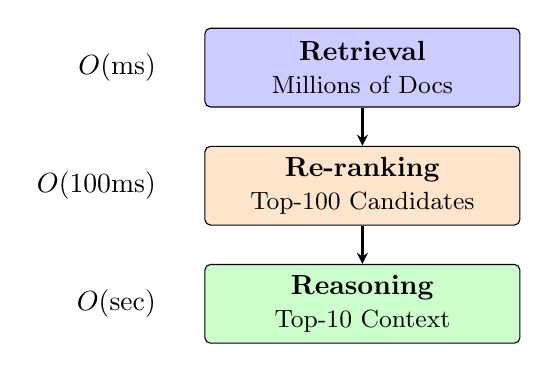
\begin{tikzpicture}[
    box/.style={rectangle, draw, fill=#1!20, minimum width=4cm, minimum height=1cm, align=center, rounded corners=2pt},
    arrow/.style={->, >=stealth, thick}
]
    % Pipeline Steps
    \node[box=blue] (ret) at (0,3) {\textbf{Retrieval}\\{\small Millions of Docs}};
    \node[box=orange] (rank) at (0,1.5) {\textbf{Re-ranking}\\{\small Top-100 Candidates}};
    \node[box=green] (llm) at (0,0) {\textbf{Reasoning}\\{\small Top-10 Context}};
    
    % Connections
    \draw[arrow] (ret) -- (rank);
    \draw[arrow] (rank) -- (llm);
    
    % Latency Annotations
    \node[anchor=east] at (-2.5, 3) {$O(\text{ms})$};
    \node[anchor=east] at (-2.5, 1.5) {$O(100\text{ms})$};
    \node[anchor=east] at (-2.5, 0) {$O(\text{sec})$};
\end{tikzpicture}

\end{center}

\begin{definition}[Traditional Retrieval]
\label{def:traditional-retrieval}
Traditional retrieval is a paradigm in which a user issues a keyword query and the system returns a ranked list of documents. The user is responsible for reading, evaluating, and synthesizing the returned results.
\end{definition}

Traditional search engines (Google, Bing, Yahoo circa 2000s) exemplify this model. The user receives a ranked list of documents and must click through links and read to find the answer.

\begin{center}
\begin{tikzpicture}[scale=0.8, every node/.style={transform shape}]
    % Mock browser
    \draw[thick, fill=gray!10] (0,0) rectangle (5,4);
    \draw[thick] (0,3.5) -- (5,3.5);
    \node at (2.5, 3.75) {\tiny browser.com};
    
    % Search bar
    \draw[fill=white] (0.5, 3) rectangle (4.5, 3.3);
    \node at (1, 3.15) {\tiny \faSearch \textit{what is IR?}};
    
    % Results
    \foreach \y in {0.5, 1.2, 1.9, 2.6} {
        \draw[blue, thick] (0.5, \y+0.2) -- (4, \y+0.2);
        \draw[gray!50] (0.5, \y) -- (3, \y);
    }
\end{tikzpicture}

\end{center}

\begin{definition}[Retrieval-Augmented Generation (RAG)]
\label{def:rag}
Retrieval-Augmented Generation (RAG) is a paradigm in which a retrieval system first fetches relevant passages from a document collection, augments a large language model (LLM) prompt with these passages, and the LLM generates a synthesized natural-language answer~\cite{lewis2020rag}.
\end{definition}

\begin{center}
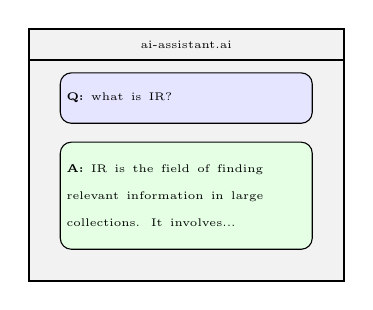
\begin{tikzpicture}[scale=0.8, every node/.style={transform shape}]
    % Mock chat
    \draw[thick, fill=gray!10] (0,0) rectangle (5,4);
    \draw[thick] (0,3.5) -- (5,3.5);
    \node at (2.5, 3.75) {\tiny ai-assistant.ai};
    
    % Chat bubble
    \draw[fill=blue!10, rounded corners] (0.5, 2.5) rectangle (4.5, 3.3);
    \node[text width=3.8cm] at (2.5, 2.9) {\tiny \textbf{Q:} what is IR?};
    
    % Answer bubble
    \draw[fill=green!10, rounded corners] (0.5, 0.5) rectangle (4.5, 2.2);
    \node[text width=3.8cm] at (2.5, 1.35) {\tiny \textbf{A:} IR is the field of finding relevant information in large collections. It involves...};
\end{tikzpicture}

\end{center}

The RAG process consists of three stages:
\begin{enumerate}
    \item \textbf{Retrieve} relevant passages from an index.
    \item \textbf{Augment} the LLM prompt with retrieved content.
    \item \textbf{Generate} a final answer using the LLM.
\end{enumerate}

Modern systems such as ChatGPT (with browsing), Perplexity, and Bing Chat follow this pattern.

\subsection{The Interface Changed, the Engine Did Not}

\begin{center}
\begin{center}
\begin{minipage}{0.45\textwidth}
\centering
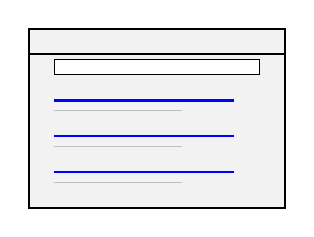
\begin{tikzpicture}[scale=0.65, every node/.style={transform shape}]
    % Mock browser
    \draw[thick, fill=gray!10] (0,0) rectangle (5,3.5);
    \draw[thick] (0,3) -- (5,3);
    \draw[fill=white] (0.5, 2.6) rectangle (4.5, 2.9);
    \foreach \y in {0.5, 1.2, 1.9} {
        \draw[blue, thick] (0.5, \y+0.2) -- (4, \y+0.2);
        \draw[gray!50] (0.5, \y) -- (3, \y);
    }
\end{tikzpicture}

\end{minipage}
\hfill
\begin{minipage}{0.45\textwidth}
\centering
\begin{tikzpicture}[scale=0.65, every node/.style={transform shape}]
    % Mock chat
    \draw[thick, fill=gray!10] (0,0) rectangle (5,3.5);
    \draw[thick] (0,3) -- (5,3);
    \draw[fill=blue!10, rounded corners] (0.5, 2.4) rectangle (4.5, 2.9);
    \node at (2.5, 2.65) {\tiny \faUser \textit{ what is IR?}};
    \draw[fill=green!10, rounded corners] (0.5, 0.5) rectangle (4.5, 1.8);
    \node[text width=3.8cm] at (2.5, 1.15) {\tiny \faRobot \textbf{A:} IR is the field of finding relevant information...};
\end{tikzpicture}

\end{minipage}
\end{center}
\end{center}

\begin{keytakeaway}
\textbf{Retrieval now serves models instead of users.} In RAG systems, the retrieval component acts as the LLM's ``eyes'' into the document collection. The underlying components---indexing, retrieval, and relevance scoring---remain the same whether we serve 10 blue links or a generated answer.
\end{keytakeaway}

\subsection{Why Indexing Matters}

Indexing is the process of organizing a document collection into a data structure that enables efficient retrieval. Without indexing, every query would require scanning the entire collection.

\begin{center}
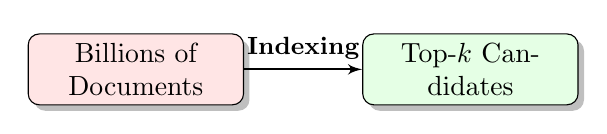
\begin{tikzpicture}[
    node distance=1.5cm,
    box/.style={rectangle, draw, rounded corners, fill=blue!15, text width=2.5cm, align=center, minimum height=0.8cm, drop shadow},
    arrow/.style={->, thick, >=latex'}
]
    \node[box, fill=red!10] (all) {Billions of Documents};
    \node[box, right=of all, fill=green!10] (few) {Top-$k$ Candidates};
    \draw[arrow] (all) -- node[above, font=\small\bf] {Indexing} (few);
\end{tikzpicture}

\end{center}

Three reasons make indexing indispensable:
\begin{enumerate}
    \item \textbf{Scale:} We cannot score every document for every query in real time.
    \item \textbf{Latency:} Users and LLMs expect sub-second responses.
    \item \textbf{Feasibility:} We must reduce millions of documents to hundreds of candidates.
\end{enumerate}

\begin{definition}[Recall Ceiling]
\label{def:recall-ceiling}
The \emph{recall ceiling} of an indexing system is the maximum recall achievable by any downstream component. If a relevant document is not returned by the candidate generation stage, no re-ranker or LLM can recover it.
\end{definition}

\begin{center}
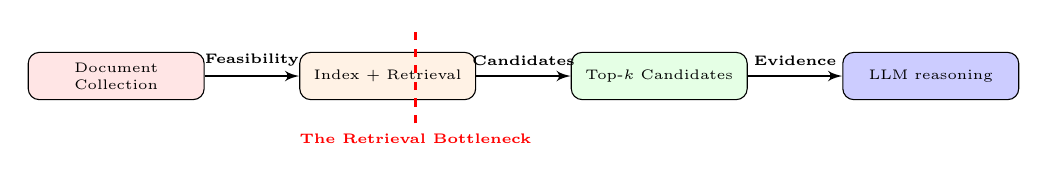
\begin{tikzpicture}[
    node distance=1.2cm,
    box/.style={rectangle, draw, rounded corners, fill=blue!10, text width=2cm, align=center, minimum height=0.6cm, font=\tiny},
    arrow/.style={->, thick, >=latex'}
]
    \node[box, fill=red!10] (coll) {Document Collection};
    \node[box, right=of coll, fill=orange!10] (idx) {Index + Retrieval};
    \node[box, right=of idx, fill=green!10] (top) {Top-$k$ Candidates};
    \node[box, right=of top, fill=blue!20] (llm) {LLM reasoning};
    
    \draw[arrow] (coll) -- node[above, font=\tiny\bf] {Feasibility} (idx);
    \draw[arrow] (idx) -- node[above, font=\tiny\bf] {Candidates} (top);
    \draw[arrow] (top) -- node[above, font=\tiny\bf] {Evidence} (llm);
    
    \draw[dashed, red, thick] (3.8, -0.6) -- (3.8, 0.6) node[below=1.2cm, font=\tiny\bf, text=red] {The Retrieval Bottleneck};
\end{tikzpicture}

\end{center}

\begin{keytakeaway}
\textbf{Indexing is not just an optimization---it is the bridge to feasibility.} If retrieval misses a document, the LLM cannot reason about it.
\end{keytakeaway}

\subsection{Course Context}

This lecture sits in the following sequence: (1)~Introduction to IR: VSM \& Boolean Retrieval; (2)~\textbf{Modern Indexing for RAG} $\leftarrow$ Today; (3)~Ranking: BM25, Query Expansion, Language Models; (4)~Embeddings \& Transformer Re-rankers; (5)~Dense Retrieval Deep Dive; (6)~Learning to Rank.

%=======================================================================
\section{Sparse Indexing: The Classical Approach}
\label{sec:sparse}
%=======================================================================

\subsection{The Inverted Index}

The inverted index is the foundational data structure of text retrieval, powering Google Search, Elasticsearch, OpenSearch, PostgreSQL full-text search, and the sparse component of virtually every RAG system in production.

\begin{definition}[Inverted Index]
\label{def:inverted-index}
An \emph{inverted index} is a data structure that maps each term $t$ in the vocabulary $V$ to a \emph{posting list}---an ordered list of document identifiers (and optionally term frequencies and positions) in which term $t$ appears:
\[
\mathrm{InvertedIndex}: V \to \{(d_1, \mathrm{payload}_1), (d_2, \mathrm{payload}_2), \ldots\}
\]
where each $d_i$ is a document identifier and $\mathrm{payload}_i$ may contain the term frequency $\mathrm{tf}(t, d_i)$, positional information, or other metadata~\cite{manning2008introduction}.
\end{definition}

Why still relevant in the age of neural networks?
\begin{enumerate}
    \item \textbf{Exact matching:} Finds ``iPhone 15 Pro Max'' precisely.
    \item \textbf{Speed:} 5--10\,ms queries over millions of documents.
    \item \textbf{Explainability:} Can inspect which terms matched.
    \item \textbf{Hybrid search:} Complements dense retrieval.
\end{enumerate}

\subsubsection{Worked Example: Building an Inverted Index}

\begin{example}[Constructing an Inverted Index]
\label{ex:inverted-index}
Consider three documents:
\begin{itemize}[nosep]
    \item \textbf{Doc 1:} ``neural networks for deep learning''
    \item \textbf{Doc 2:} ``deep learning applications''
    \item \textbf{Doc 3:} ``neural machine translation''
\end{itemize}

\begin{center}
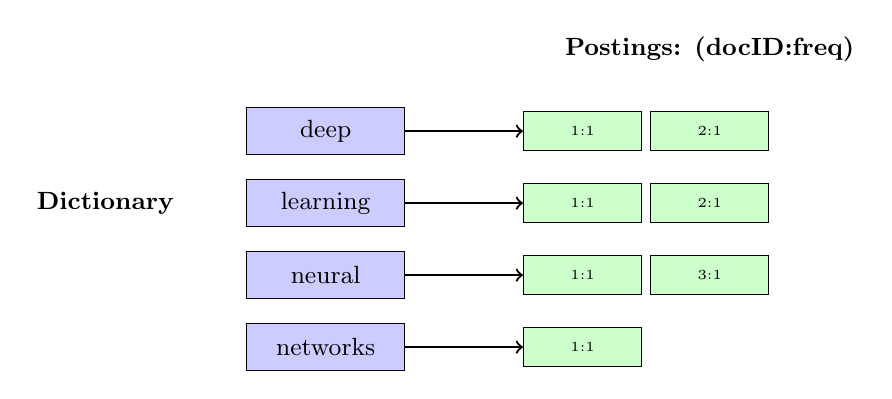
\begin{tikzpicture}[
    node distance=0.3cm,
    dict/.style={rectangle, draw, fill=blue!20, minimum width=2cm, minimum height=0.6cm, font=\small},
    post/.style={rectangle, draw, fill=green!20, minimum width=1.5cm, minimum height=0.5cm, font=\tiny}
]
    % Dictionary
    \node[dict] (t1) {deep};
    \node[dict, below=of t1] (t2) {learning};
    \node[dict, below=of t2] (t3) {neural};
    \node[dict, below=of t3] (t4) {networks};
    
    \node[left=0.8cm of t2.west, font=\small\bf] {Dictionary};
    
    % Postings
    \node[post, right=1.5cm of t1] (p11) {1:1};
    \node[post, right=0.1cm of p11] (p12) {2:1};
    
    \node[post, right=1.5cm of t2] (p21) {1:1};
    \node[post, right=0.1cm of p21] (p22) {2:1};
    
    \node[post, right=1.5cm of t3] (p31) {1:1};
    \node[post, right=0.1cm of p31] (p32) {3:1};
    
    \node[post, right=1.5cm of t4] (p41) {1:1};
    
    \node[above=0.5cm of p12, font=\small\bf] {Postings: (docID:freq)};
    
    % Arrows
    \draw[->, thick] (t1) -- (p11);
    \draw[->, thick] (t2) -- (p21);
    \draw[->, thick] (t3) -- (p31);
    \draw[->, thick] (t4) -- (p41);
\end{tikzpicture}

\end{center}

After tokenization and lowercasing, the inverted index is:

\begin{center}
\begin{tabular}{ll}
\toprule
\textbf{Term} & \textbf{Posting List} \\
\midrule
neural & $[1, 3]$ \\
networks & $[1]$ \\
for & $[1]$ \\
deep & $[1, 2]$ \\
learning & $[1, 2]$ \\
applications & $[2]$ \\
machine & $[3]$ \\
translation & $[3]$ \\
\bottomrule
\end{tabular}
\end{center}

\textbf{Query Processing} for ``neural learning'':
\begin{enumerate}[nosep]
    \item Look up ``neural'' $\to [1, 3]$.
    \item Look up ``learning'' $\to [1, 2]$.
    \item Intersect: $[1, 3] \cap [1, 2] = [1]$.
    \item Result: Document~1 contains both terms.
\end{enumerate}
\end{example}

\subsection{The Inverted Index as a Sparse Matrix}

\begin{definition}[Document-Term Matrix]
\label{def:doc-term-matrix}
The \emph{document-term matrix} $\mathbf{M} \in \mathbb{R}^{D \times |V|}$ has rows for documents, columns for vocabulary terms, and entries $\mathbf{M}_{i,j}$ containing the weight (TF-IDF, BM25) of term $j$ in document $i$. This matrix is extremely sparse---typically $>$99.9\% zeros.
\end{definition}

\begin{center}
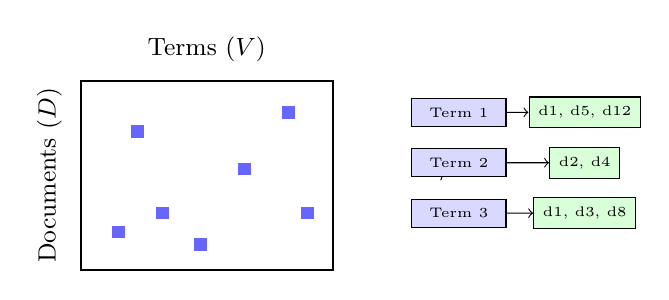
\begin{tikzpicture}[scale=0.8]
    % Matrix outline
    \draw[thick] (0,0) rectangle (4,3);
    \node[rotate=90] at (-0.5, 1.5) {\small Documents ($D$)};
    \node at (2, 3.5) {\small Terms ($V$)};
    
    % Sparse points
    \foreach \x/\y in {0.5/0.5, 1.2/0.8, 0.8/2.1, 2.5/1.5, 3.2/2.4, 1.8/0.3, 3.5/0.8} {
        \fill[blue!60] (\x, \y) rectangle (\x+0.2, \y+0.2);
    }
    
    \node[right=4.2cm] at (0, 1.5) {$\rightarrow$};
    
    % Index structure
    \begin{scope}[shift={(6,0.5)}]
        \node[draw, fill=blue!15, minimum width=1.2cm] (t1) at (0, 2) {\tiny Term 1};
        \node[draw, fill=blue!15, minimum width=1.2cm] (t2) at (0, 1.2) {\tiny Term 2};
        \node[draw, fill=blue!15, minimum width=1.2cm] (t3) at (0, 0.4) {\tiny Term 3};
        
        \node[draw, fill=green!15] (p1) at (2, 2) {\tiny d1, d5, d12};
        \node[draw, fill=green!15] (p2) at (2, 1.2) {\tiny d2, d4};
        \node[draw, fill=green!15] (p3) at (2, 0.4) {\tiny d1, d3, d8};
        
        \draw[->] (t1) -- (p1);
        \draw[->] (t2) -- (p2);
        \draw[->] (t3) -- (p3);
    \end{scope}
\end{tikzpicture}

\end{center}

\begin{keytakeaway}
The inverted index is a \textbf{Compressed Sparse Column (CSC)} storage format of the document-term matrix. We store only non-zero entries, avoiding the full $D \times |V|$ cost.
\end{keytakeaway}

\subsection{Complexity Analysis}

\begin{proposition}[Complexity of Inverted Index Retrieval]
Given $N$ documents with average length $M$, a query of $k$ terms, and average posting list length $p$:
\begin{itemize}[nosep]
    \item \textbf{Naive scan:} $O(N \cdot M)$.
    \item \textbf{Inverted index:} $O(k \cdot p)$, where typically $k \ll N$ and $p \ll N$.
\end{itemize}
\end{proposition}

\begin{example}[Speed Comparison]
For 10M documents $\times$ 500 words: naive requires $5 \times 10^9$ comparisons. For query ``neural learning'' ($k=2$, $p \approx 1000$): inverted index needs $\sim$2000 comparisons---\textbf{$\sim$1000$\times$ faster}.
\end{example}

\subsection{Posting List Formats}

\begin{definition}[Posting List Levels]
\label{def:posting-levels}
\leavevmode
\begin{enumerate}
    \item \textbf{Level 1 --- DocID Only (Boolean Retrieval):} $t \to [d_1, d_2, \ldots]$. Supports AND/OR/NOT but no ranking.
    \item \textbf{Level 2 --- With Frequencies (Ranked Retrieval):} $t \to [(d_1, \mathrm{tf}_1), (d_2, \mathrm{tf}_2), \ldots]$. Supports TF-IDF, BM25. \textbf{Standard in practice.}
    \item \textbf{Level 3 --- With Positions (Phrase Queries):} $t \to [(d_1, \mathrm{tf}_1, [\mathrm{pos}_{1,1}, \ldots]), \ldots]$. Supports exact phrases and proximity scoring. 2--3$\times$ larger.
\end{enumerate}
\end{definition}

\begin{example}[Posting List Formats]
For the term ``neural'':
\begin{itemize}[nosep]
    \item \textbf{Level 1:} \texttt{neural: [1, 3, 5, 12, 27, 89]}
    \item \textbf{Level 2:} \texttt{neural: [(1,tf=2), (3,tf=1), (5,tf=3), ...]}
    \item \textbf{Level 3:} \texttt{neural: [(1,tf=2,pos=[5,42]), (3,tf=1,pos=[8]), ...]}
\end{itemize}
\end{example}

\subsection{Score Aggregation and the Vector Space Model}

\begin{definition}[Vector Space Model Scoring]
\label{def:vsm-scoring}
In the Vector Space Model~\cite{salton1975vector}, relevance is:
\begin{equation}
\mathrm{score}(q, d) = \sum_{t \in q \cap d} w(t, q) \times w(t, d)
\label{eq:vsm}
\end{equation}
where $w(t, q)$ and $w(t, d)$ are term weights in query and document (e.g., TF-IDF).
\end{definition}

The engine uses \emph{accumulators}:
\begin{enumerate}[nosep]
    \item Initialize $\mathrm{Acc}[d] = 0$ for all $d$.
    \item For each query term $t$, traverse its posting list; for each $(d, \mathrm{tf})$: $\mathrm{Acc}[d] \mathrel{+}= w(t,q) \times w(t,d)$.
    \item Return documents sorted by $\mathrm{Acc}[d]$.
\end{enumerate}

\begin{center}
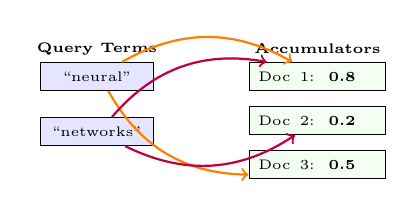
\begin{tikzpicture}[scale=0.7]
    \node[font=\bf\tiny] at (1, 3.5) {Query Terms};
    \node[draw, fill=blue!10, text width=1.2cm, align=center] (q1) at (1, 3) {\tiny ``neural''};
    \node[draw, fill=blue!10, text width=1.2cm, align=center] (q2) at (1, 2) {\tiny ``networks''};
    
    \node[font=\bf\tiny] at (5, 3.5) {Accumulators};
    \node[draw, fill=green!5, text width=1.5cm] (a1) at (5, 3) {\tiny Doc 1: \textbf{0.8}};
    \node[draw, fill=green!5, text width=1.5cm] (a2) at (5, 2.2) {\tiny Doc 2: \textbf{0.2}};
    \node[draw, fill=green!5, text width=1.5cm] (a3) at (5, 1.4) {\tiny Doc 3: \textbf{0.5}};
    
    \draw[->, orange, thick] (q1) to[bend left] (a1);
    \draw[->, orange, thick] (q1) to[bend right] (a3);
    \draw[->, purple, thick] (q2) to[bend left] (a1);
    \draw[->, purple, thick] (q2) to[bend right] (a2);
\end{tikzpicture}

\end{center}

\begin{keytakeaway}
Sparse indexing computes scores \textbf{only for documents containing at least one query term}. All others are never touched.
\end{keytakeaway}

\subsection{Text Preprocessing Pipeline}
\label{sec:preprocessing}

The same preprocessing must be applied to both documents and queries.

\begin{center}
\begin{tikzpicture}[scale=0.6, transform shape, spacing/.style={yshift=-2.5cm}]
    % Sequential Boxes using API
    \IRBox{raw}{(0,0)}{The Neural Networks \\ are Learning!}{String Input}{accent}
    
    \begin{scope}[spacing]
        \IRBox{token}{($ (raw) + (0,-2.5) $)}{[The, Neural, Networks, \\ are, Learning, !]}{Tokenized}{primary}
        \IRBox{lower}{($ (token) + (0,-2.5) $)}{[the, neural, networks, \\ are, learning, !]}{Normalized}{primary}
        \IRBox{stop}{($ (lower) + (0,-2.5) $)}{[neural, networks, \\ learning]}{Filtered}{primary}
        \IRBox{stem}{($ (stop) + (0,-2.5) $)}{[neural, network, \\ learn]}{Stemmed}{emph}
    \end{scope}

    % Connect with sloped labels using TB arrows for vertical flow
    \IRArrowTB{raw}{token}{Tokenize}
    \IRArrowTB{token}{lower}{Lowercase}
    \IRArrowTB{lower}{stop}{Stopwords}
    \IRArrowTB{stop}{stem}{Stem/Lemmatize}
\end{tikzpicture}

\end{center}

\begin{example}[Preprocessing Pipeline]
\textbf{Raw:} ``The Neural Networks are Learning!''
\begin{enumerate}[nosep]
    \item \textbf{Tokenize:} [``The'', ``Neural'', ``Networks'', ``are'', ``Learning'', ``!'']
    \item \textbf{Lowercase:} [``the'', ``neural'', ``networks'', ``are'', ``learning'', ``!'']
    \item \textbf{Remove stop words:} [``neural'', ``networks'', ``learning'']
    \item \textbf{Stem (Porter):} [``neural'', ``network'', ``learn'']
\end{enumerate}
\end{example}

\subsubsection{Tokenization}

\begin{definition}[Tokenization]
\emph{Tokenization} segments text into discrete tokens (words or subwords), defining the index vocabulary.
\end{definition}

Language-specific challenges: English contractions (``don't''), German compounds (``Informationssystem''), Chinese/Japanese (no whitespace).

\subsubsection{Stemming vs.\ Lemmatization}

\begin{definition}[Stemming]
\emph{Stemming} reduces words to approximate root forms by removing suffixes heuristically (e.g., Porter's algorithm~\cite{porter1980algorithm}).
\end{definition}

\begin{definition}[Lemmatization]
\emph{Lemmatization} reduces words to their dictionary form (lemma) using morphological analysis, producing valid words.
\end{definition}

\begin{example}[Stemming vs.\ Lemmatization]
\begin{center}
\begin{tabular}{lll}
\toprule
\textbf{Word} & \textbf{Porter Stemmer} & \textbf{Lemmatizer} \\
\midrule
running & run & run \\
better & better & good \\
university & univers \textcolor{red}{(wrong)} & university \\
studies & studi & study \\
\bottomrule
\end{tabular}
\end{center}
\end{example}

\begin{pitfall}
\textbf{Do NOT stem for neural models.} BERT and sentence-transformers expect natural text. Stemming destroys subword information these models depend on.
\end{pitfall}

\subsubsection{Stop Words}

\begin{definition}[Stop Words]
\emph{Stop words} are high-frequency words (``the'', ``a'', ``is'') carrying little discriminative information.
\end{definition}

\textbf{Modern recommendation: keep stop words} unless you have a specific reason to remove them. Storage is cheap, stop words matter for phrases (``to be or not to be''), entity names (``The Who''), and neural models.

\subsubsection{Preprocessing Depends on Representation}

\begin{center}
\begin{tabular}{lll}
\toprule
\textbf{Step} & \textbf{Sparse Retrieval} & \textbf{Dense Retrieval} \\
\midrule
Tokenization & Custom (vocabulary) & Fixed by model (BPE, WordPiece) \\
Stemming & Useful & \textbf{Not used} \\
Stop words & Optional & Kept \\
Truncation & N/A & Critical (context window) \\
\bottomrule
\end{tabular}
\end{center}

\begin{center}
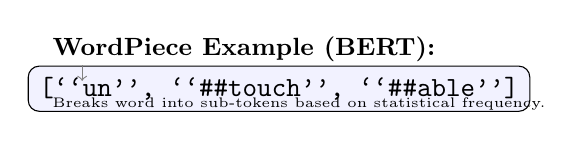
\begin{tikzpicture}
    % WordPiece example
    \node[anchor=west] at (0, 0.5) {\small \textbf{WordPiece Example (BERT):}};
    \node[draw, fill=blue!5, rounded corners, inner sep=4pt] at (3, 0) {\texttt{[``un'', ``\#\#touch'', ``\#\#able'']}};
    \draw[->, gray, thin] (0.5, 0.3) -- (0.5, 0.1);
    \node[anchor=west] at (0, -0.2) {\tiny Breaks word into sub-tokens based on statistical frequency.};
\end{tikzpicture}

\end{center}

\subsection{Index Compression}
\label{sec:compression}

Compression is not optional---it makes systems both \textbf{faster} and cheaper. CPUs decompress at 2--5~GB/s while SSDs read at $\sim$0.5~GB/s, so reading compressed data is faster than reading uncompressed data.

\subsubsection{Gap Encoding}

\begin{definition}[Gap Encoding]
\emph{Gap encoding} (delta encoding) replaces an ordered posting list $[d_1, d_2, \ldots, d_n]$ with gaps $[d_1, d_2 - d_1, d_3 - d_2, \ldots, d_n - d_{n-1}]$. Gaps are typically small, requiring fewer bits~\cite{manning2008introduction}.
\end{definition}

\begin{example}[Gap Encoding]
\textbf{Original:} $[5, 127, 214, 215, 512, 1024, 2048, 10239]$

\textbf{Gaps:} $[5, 122, 87, 1, 297, 512, 1024, 8191]$

Original values need 14 bits each (range up to 10,239). Most gaps are $<256$ (8 bits)---much better compression. Decoding is sequential: $d_i = d_{i-1} + \mathrm{gap}_i$.
\end{example}

\subsubsection{Variable Byte (VB) Encoding}

\begin{definition}[Variable Byte Encoding]
\emph{Variable Byte (VB) encoding} represents each integer using a variable number of bytes: 7 bits per byte for data, 1 bit (MSB) as continuation flag. MSB$=1$: last byte; MSB$=0$: more bytes follow.
\end{definition}

\begin{example}[VB Encoding Step-by-Step]
\label{ex:vb}

\textbf{Encode 5:} Binary \texttt{101} (3 bits $\leq$ 7). VB: \texttt{1\_0000101} (1 byte).

\textbf{Encode 122:} Binary \texttt{1111010} (7 bits $\leq$ 7). VB: \texttt{1\_1111010} (1 byte).

\textbf{Encode 824:}
\begin{enumerate}[nosep]
    \item Binary: \texttt{1100111000} (10 bits, needs 2 bytes since $10 > 7$).
    \item Split into 7-bit chunks from right: lower = \texttt{0111000}, upper = \texttt{0000110}.
    \item Byte 1 (upper): \texttt{0\_0000110} (continuation$=0$, more follows).
    \item Byte 2 (lower): \texttt{1\_0111000} (continuation$=1$, last byte).
    \item Result: \texttt{00000110\;10111000} (2 bytes).
\end{enumerate}

\textbf{Decode 824:}
\begin{enumerate}[nosep]
    \item Read bytes until MSB$=1$: \texttt{00000110}, \texttt{10111000}.
    \item Strip MSBs: \texttt{0000110}, \texttt{0111000}.
    \item Concatenate: \texttt{0000110\_0111000} $= 1100111000_2 = 824$.
\end{enumerate}

\textbf{Compression:} Gaps $[5, 122, 87, 1]$ need 4~bytes (VB) vs.\ 16~bytes (32-bit ints) --- \textbf{4$\times$ compression}.
\end{example}

\subsubsection{Compression in Practice}

\begin{center}
\begin{tabular}{ll}
\toprule
\textbf{Method} & \textbf{Typical Compression} \\
\midrule
Variable Byte (VB) & 3--4$\times$ \\
PForDelta & 6--10$\times$ \\
Dictionary (front coding) & 30--50\% savings \\
\bottomrule
\end{tabular}
\end{center}

\begin{production}
\textbf{Lucene/Elasticsearch:} FOR with SIMD. \textbf{Google:} Custom hardware-optimized. \textbf{Your projects:} VB encoding is sufficient---simple and effective.
\end{production}

\subsection{PyTerrier: Sparse Indexing in Practice}

\begin{lstlisting}[caption={Sparse indexing and BM25 retrieval with PyTerrier~\cite{macdonald2021pyterrier}.}]
import pyterrier as pt
pt.init()

dataset = pt.get_dataset('irds:vaswani')
indexer = pt.IterDictIndexer("./vaswani_index", overwrite=True)
index_ref = indexer.index(dataset.get_corpus_iter())

bm25 = pt.BatchRetrieve(index_ref, wmodel="BM25")
results = bm25.search("aerodynamic flow over wings")
print(results[['docno', 'score', 'rank']].head())

evaluation = pt.Experiment(
    [bm25], dataset.get_topics(), dataset.get_qrels(),
    eval_metrics=["map", "ndcg_cut_10", "P_10"])
print(evaluation)
\end{lstlisting}

%=======================================================================
\section{Dense Vector Indexing for Neural Retrieval}
\label{sec:dense}
%=======================================================================

\subsection{The Shift to Dense Vectors}

\begin{definition}[Sparse Representation]
A \emph{sparse representation} of a document is a vector $\vec{d} \in \mathbb{R}^{|V|}$ over the vocabulary, where most entries are zero. Only terms present in the document have non-zero weights.
\end{definition}

\begin{definition}[Dense Representation (Embedding)]
A \emph{dense representation} is a vector $\vec{d} \in \mathbb{R}^{d}$ (typically $d = 768$) produced by a neural encoder (e.g., BERT, sentence-transformers~\cite{reimers2019sentence}), where \textbf{all entries are non-zero} and encode semantic meaning.
\end{definition}

\begin{center}
\begin{tabular}{lll}
\toprule
& \textbf{Sparse (BM25)} & \textbf{Dense (Neural)} \\
\midrule
Dimensionality & $\sim$30,000 & 768 \\
Sparsity & $>$99.99\% zeros & 100\% non-zero \\
Matching & Lexical (exact words) & Semantic (meaning) \\
``car problems'' vs.\ ``automobile issues'' & \textcolor{red}{No match} & \textcolor{green}{Match} \\
\bottomrule
\end{tabular}
\end{center}

Dense vectors cannot use inverted indexes (no discrete terms). We need \textbf{Approximate Nearest Neighbor (ANN)} search.

\begin{center}
\begin{tikzpicture}[scale=0.5, every node/.style={scale=0.5}]
    % Raw Input
    \IRBox{text}{(0,0)}{Raw Text}{Collection}{primary}
    
    % Sparse branch
    \IRBox{tokens}{(4,1.5)}{Tokenization}{Lexical Phase}{primary}
    \IRBox{ids}{(8,1.5)}{Term IDs}{Mapping}{primary}
    \IRBox{sindex}{(12,1.5)}{Inverted Index}{Static Index}{secondary}
    
    % Dense branch
    \IRBox{mtoken}{(4,-1.5)}{Model Tokenizer}{Neural Phase}{accent}
    \IRBox{embed}{(8,-1.5)}{Encoding (BERT)}{Vectorization}{accent}
    \IRBox{dindex}{(12,-1.5)}{ANN Index}{Dynamic Index}{secondary}
    
    % Target
    \IRBox{res}{(16,0)}{Ranked Candidates}{Top-$k$ List}{emph}
    
    % Sparse Connections
    \IRArrow{text.north}{tokens.west}{Sparse Pipeline}
    \IRArrow{tokens}{ids}{}
    \IRArrow{ids}{sindex}{}
    \IRArrow{sindex}{res.north}{}
    
    % Dense Connections
    \IRArrow{text.south}{mtoken.west}{Dense Pipeline}
    \IRArrow{mtoken}{embed}{}
    \IRArrow{embed}{dindex}{}
    \IRArrow{dindex}{res.south}{}
\end{tikzpicture}

\end{center}

\subsection{The ANN Search Problem}

\begin{definition}[Nearest Neighbor Search]
Given $N$ vectors $\mathcal{D} = \{\vec{d}_1, \ldots, \vec{d}_N\} \subset \mathbb{R}^d$ and query $\vec{q} \in \mathbb{R}^d$, the $k$-NN problem finds $\mathcal{S}^* \subset \mathcal{D}$ with $|\mathcal{S}^*| = k$ such that $\forall \vec{d} \in \mathcal{S}^*,\; \forall \vec{d}' \in \mathcal{D} \setminus \mathcal{S}^*: \mathrm{sim}(\vec{q}, \vec{d}) \geq \mathrm{sim}(\vec{q}, \vec{d}')$.
\end{definition}

\begin{definition}[Approximate Nearest Neighbor (ANN)]
ANN search relaxes exactness, returning $\hat{\mathcal{S}}$ such that $|\hat{\mathcal{S}} \cap \mathcal{S}^*|/k \geq 1 - \epsilon$ with high probability, trading recall for speed~\cite{indyk1998approximate}.
\end{definition}

\textbf{Why exact search is infeasible:} For $N = 10^9$, $d = 768$: brute-force needs $\sim$768 billion FLOPs per query ($>$1s even on GPU).

\begin{center}
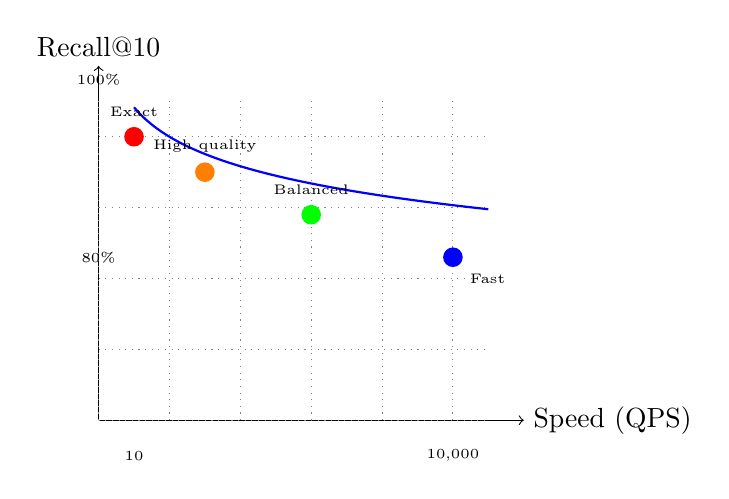
\begin{tikzpicture}[scale=0.9]
    % Axes
    \draw[->] (0,0) -- (6,0) node[right] {Speed (QPS)};
    \draw[->] (0,0) -- (0,5) node[above] {Recall@10};
    
    % Grid
    \draw[gray, dotted] (0,0) grid (5.5,4.5);
    
    % Curve
    \draw[blue, thick, domain=0.5:5.5, samples=100] 
        plot (\x, {4 - 0.6*ln(\x)});
    
    % Points
    \node[circle, fill=red, inner sep=2.5pt, label=above:{\tiny Exact}] at (0.5, 4) {};
    \node[circle, fill=orange, inner sep=2.5pt, label=above:{\tiny High quality}] at (1.5, 3.5) {};
    \node[circle, fill=green, inner sep=2.5pt, label=above:{\tiny Balanced}] at (3, 2.9) {};
    \node[circle, fill=blue, inner sep=2.5pt, label=below right:{\tiny Fast}] at (5, 2.3) {};
    
    % Labels
    \node at (0, 4.8) {\tiny 100\%};
    \node at (0, 2.3) {\tiny 80\%};
    \node at (0.5, -0.5) {\tiny 10};
    \node at (5, -0.5) {\tiny 10,000};
\end{tikzpicture}

\end{center}

Typical operating points:
\begin{itemize}[nosep]
    \item \textbf{High quality:} 95--99\% recall, 100--500 QPS (production RAG).
    \item \textbf{Balanced:} 90--95\% recall, 500--2000 QPS.
    \item \textbf{Fast:} 80--90\% recall, 2000--10,000 QPS.
\end{itemize}

\subsection{IVF: Inverted File Index for Vectors}

\begin{definition}[Inverted File Index (IVF)]
The \emph{IVF} partitions the vector space into $k$ Voronoi cells via $k$-means, maintaining an inverted list per cluster. At query time, only vectors in the $n_{\mathrm{probe}}$ nearest clusters are searched~\cite{jegou2011product}.
\end{definition}

\begin{center}
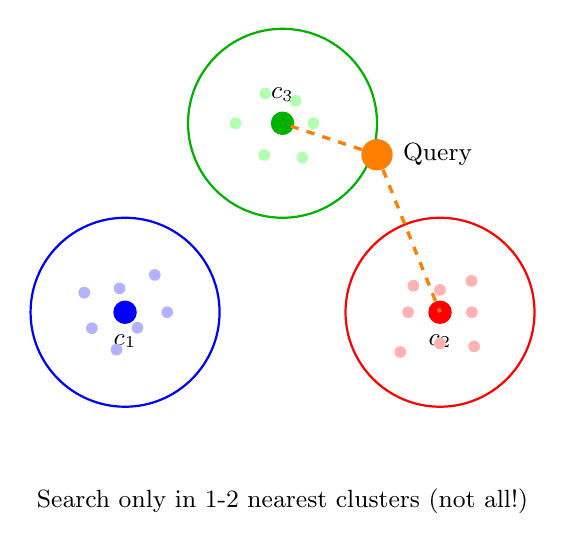
\begin{tikzpicture}[scale=0.8]
    % Cluster 1
    \draw[thick, blue] (0,0) circle (1.5);
    \node[circle, fill=blue, inner sep=3pt, label=below:{\small $c_1$}] at (0,0) {};
    \foreach \i in {1,...,7} {
        \pgfmathsetmacro{\angle}{360/7*\i}
        \pgfmathsetmacro{\r}{0.3+0.5*rnd}
        \node[circle, fill=blue!30, inner sep=1.5pt] at (\angle:\r) {};
    }
    
    % Cluster 2
    \draw[thick, red] (5,0) circle (1.5);
    \node[circle, fill=red, inner sep=3pt, label=below:{\small $c_2$}] at (5,0) {};
    \foreach \i in {1,...,8} {
        \pgfmathsetmacro{\angle}{360/8*\i}
        \pgfmathsetmacro{\r}{0.3+0.6*rnd}
        \node[circle, fill=red!30, inner sep=1.5pt] at ($(5,0)+(\angle:\r)$) {};
    }
    
    % Cluster 3
    \draw[thick, green!70!black] (2.5,3) circle (1.5);
    \node[circle, fill=green!70!black, inner sep=3pt, label=above:{\small $c_3$}] at (2.5,3) {};
    \foreach \i in {1,...,6} {
        \pgfmathsetmacro{\angle}{360/6*\i}
        \pgfmathsetmacro{\r}{0.4+0.5*rnd}
        \node[circle, fill=green!30, inner sep=1.5pt] at ($(2.5,3)+(\angle:\r)$) {};
    }
    
    % Query
    \node[circle, fill=orange, inner sep=4pt, label=right:{\small Query}] (q) at (4,2.5) {};
    
    % Distance to nearest clusters
    \draw[dashed, orange, very thick] (q) -- (2.5,3);
    \draw[dashed, orange, very thick] (q) -- (5,0);
    
    \node at (2.5,-3.0) {\small Search only in 1-2 nearest clusters (not all!)};
\end{tikzpicture}

\end{center}

\subsubsection{IVF Construction}

\begin{algorithm}[H]
\caption{IVF Construction}
\begin{algorithmic}[1]
\REQUIRE Vectors $\mathcal{D}$, number of clusters $k$
\STATE Run $k$-means on $\mathcal{D} \to$ centers $\{\vec{c}_1, \ldots, \vec{c}_k\}$
\FOR{each $\vec{d}_i \in \mathcal{D}$}
    \STATE Assign to nearest center: $j^* = \arg\min_j \|\vec{d}_i - \vec{c}_j\|$
\ENDFOR
\STATE Build inverted lists: cluster $j \to$ [vector IDs in cluster $j$]
\end{algorithmic}
\end{algorithm}

\subsubsection{IVF Search}

\begin{algorithm}[H]
\caption{IVF Search}
\begin{algorithmic}[1]
\REQUIRE Query $\vec{q}$, probes $n_{\mathrm{probe}}$, results $k$
\STATE Compute distances $\vec{q} \to$ all centers
\STATE Select $n_{\mathrm{probe}}$ nearest centers
\STATE candidates $\gets$ []
\FOR{each selected cluster $j$}
    \STATE Fetch vectors in cluster $j$; compute exact distances to $\vec{q}$
    \STATE Append to candidates
\ENDFOR
\RETURN Top-$k$ from candidates by distance
\end{algorithmic}
\end{algorithm}

Key parameter: $n_{\mathrm{probe}}$ ($1$ = fast/low recall; $100$ = slow/high recall).

\subsection{Product Quantization (PQ)}

\begin{definition}[Product Quantization]
\emph{Product Quantization (PQ)}~\cite{jegou2011product} decomposes a $d$-dim vector into $m$ subvectors of dimension $d/m$, independently quantizes each to the nearest centroid from a codebook of $K$ centroids (typically $K=256$). The vector is stored as $m$ centroid indices ($m$ bytes for $K=256$).
\end{definition}

\begin{example}[Product Quantization]
A 768-dim vector (3072 bytes as float32). With $m = 96$, $K = 256$:
\begin{enumerate}[nosep]
    \item \textbf{Split} into 96 subvectors of 8 dims each.
    \item \textbf{Quantize} each subvector to nearest centroid (from 256 centroids per subspace).
    \item \textbf{Store} 96 centroid IDs $\times$ 1 byte = \textbf{96 bytes}.
\end{enumerate}
Compression: $3072 / 96 = $ \textbf{32$\times$}.

\textbf{Distance approximation without decompression:}
\begin{enumerate}[nosep]
    \item Precompute distance table: query subvector $\to$ all centroids ($96 \times 256 = 24{,}576$ distances, once per query).
    \item Per document: $\hat{d}(\vec{q}, \vec{d}) = \sum_{i=1}^{96} \mathrm{distTable}_i[\mathrm{code}_i(\vec{d})]$ --- only 96 lookups.
\end{enumerate}
\end{example}

Performance: 32$\times$ memory compression; 10--100$\times$ faster distances; 80--95\% recall.

\subsubsection{PQ Query Processing in Detail}

To understand how PQ answers a query, we must distinguish three phases: \emph{offline training}, \emph{offline encoding}, and \emph{online query processing}. The key innovation is the \textbf{Asymmetric Distance Computation (ADC)} trick: the query is \emph{not} quantized---only the database vectors are. This preserves query-side precision while gaining speed on the database side.

\paragraph{Phase 1: Offline Training (Learn Codebooks).}
Before any documents are indexed, PQ learns $m$ independent codebooks by running $k$-means on the training data:

\begin{enumerate}[nosep]
    \item Collect a representative sample of vectors from the corpus.
    \item Split every vector into $m$ subvectors of dimension $d^* = d/m$.
    \item For each subspace $i \in \{1, \ldots, m\}$, run $k$-means on all $i$-th subvectors to learn $K$ centroids. Denote the codebook for subspace $i$ as $\mathcal{C}_i = \{c_i^{(1)}, c_i^{(2)}, \ldots, c_i^{(K)}\}$, where each $c_i^{(j)} \in \mathbb{R}^{d^*}$.
\end{enumerate}

Result: $m$ codebooks, each containing $K$ centroids of dimension $d^*$.

\paragraph{Phase 2: Offline Encoding (Compress Database).}
Each database vector $\vec{d}$ is encoded as a tuple of $m$ centroid indices:

\begin{enumerate}[nosep]
    \item Decompose $\vec{d}$ into subvectors: $\vec{d} = [\vec{d}^{(1)}, \vec{d}^{(2)}, \ldots, \vec{d}^{(m)}]$.
    \item For each subspace $i$, find the nearest centroid: $\mathrm{code}_i(\vec{d}) = \arg\min_{j \in \{1,\ldots,K\}} \|\vec{d}^{(i)} - c_i^{(j)}\|^2$.
    \item Store the PQ code: $\mathrm{PQ}(\vec{d}) = [\mathrm{code}_1(\vec{d}),\; \mathrm{code}_2(\vec{d}),\; \ldots,\; \mathrm{code}_m(\vec{d})]$.
\end{enumerate}

Each code is an integer in $\{1, \ldots, K\}$, requiring $\lceil \log_2 K \rceil$ bits. For $K = 256$, each code is 1 byte, so the full PQ code is $m$ bytes.

\paragraph{Phase 3: Online Query Processing (ADC Search).}

\begin{definition}[Asymmetric Distance Computation (ADC)]
\label{def:adc}
In ADC, the squared Euclidean distance between the \emph{exact} query $\vec{q}$ and the \emph{quantized} database vector $\hat{\vec{d}}$ (reconstructed from PQ codes) is approximated as:
\begin{equation}
\|\vec{q} - \hat{\vec{d}}\|^2 = \sum_{i=1}^{m} \|\vec{q}^{(i)} - c_i^{(\mathrm{code}_i(\vec{d}))}\|^2
\label{eq:adc}
\end{equation}
This is \emph{asymmetric} because $\vec{q}$ is exact while $\vec{d}$ is quantized. The key insight is that each inner term $\|\vec{q}^{(i)} - c_i^{(j)}\|^2$ depends only on the query subvector and the centroid index, so it can be \textbf{precomputed into a lookup table}.
\end{definition}

The online query processing proceeds in two steps:

\textbf{Step 1: Build the Distance Lookup Table.}
For each subspace $i \in \{1, \ldots, m\}$ and each centroid $j \in \{1, \ldots, K\}$, compute:
\begin{equation}
\mathrm{DT}[i][j] = \|\vec{q}^{(i)} - c_i^{(j)}\|^2
\label{eq:distance-table}
\end{equation}

This produces an $m \times K$ table. The cost is $O(m \cdot K \cdot d^*)$ floating-point operations, computed \textbf{once per query}. For $m = 96$, $K = 256$, $d^* = 8$: this is $96 \times 256 \times 8 = 196{,}608$ FLOPs---negligible.

\textbf{Step 2: Scan and Accumulate.}
For each database vector (represented by its PQ code $[\mathrm{code}_1, \ldots, \mathrm{code}_m]$), compute the approximate distance by summing table lookups:
\begin{equation}
\hat{d}(\vec{q}, \vec{d}) = \sum_{i=1}^{m} \mathrm{DT}[i][\mathrm{code}_i(\vec{d})]
\label{eq:pq-scan}
\end{equation}

This requires only $m$ table lookups and $m-1$ additions per document---no floating-point multiplications at all.

\begin{algorithm}[H]
\caption{PQ Query Processing (Asymmetric Distance Computation)}
\label{alg:pq-query}
\begin{algorithmic}[1]
\REQUIRE Query vector $\vec{q} \in \mathbb{R}^d$, PQ codes for $N$ database vectors, codebooks $\{\mathcal{C}_1, \ldots, \mathcal{C}_m\}$, desired results $k$
\ENSURE Top-$k$ nearest neighbors (approximate)

\medskip
\STATE \textbf{// Step 1: Build distance lookup table (once per query)}
\STATE Decompose $\vec{q}$ into subvectors: $\vec{q}^{(1)}, \vec{q}^{(2)}, \ldots, \vec{q}^{(m)}$
\FOR{$i = 1$ to $m$}
    \FOR{$j = 1$ to $K$}
        \STATE $\mathrm{DT}[i][j] \gets \|\vec{q}^{(i)} - c_i^{(j)}\|^2$ \hfill $\triangleright$ squared L2 in $\mathbb{R}^{d^*}$
    \ENDFOR
\ENDFOR

\medskip
\STATE \textbf{// Step 2: Scan all PQ codes, accumulate distances}
\FOR{each document $n = 1$ to $N$}
    \STATE $\mathrm{dist}[n] \gets 0$
    \FOR{$i = 1$ to $m$}
        \STATE $\mathrm{dist}[n] \gets \mathrm{dist}[n] + \mathrm{DT}[i][\mathrm{code}_i^{(n)}]$ \hfill $\triangleright$ one table lookup
    \ENDFOR
\ENDFOR

\medskip
\STATE \textbf{// Step 3: Return top-$k$ by smallest distance}
\RETURN $k$ documents with smallest $\mathrm{dist}[n]$
\end{algorithmic}
\end{algorithm}

\begin{remark}[Complexity Analysis]
\leavevmode
\begin{itemize}[nosep]
    \item \textbf{Table construction (Step 1):} $O(m \cdot K \cdot d^*)$. For $m=96$, $K=256$, $d^*=8$: $\sim$197K FLOPs.
    \item \textbf{Distance scan (Step 2):} $O(N \cdot m)$ \textbf{integer} lookups + additions. For $N = 1\text{M}$, $m = 96$: 96M lookups.
    \item \textbf{Exact brute-force:} $O(N \cdot d)$ \textbf{float} multiply-adds. For $N = 1\text{M}$, $d = 768$: 768M FLOPs.
    \item \textbf{Speedup:} PQ replaces $d = 768$ float multiply-adds per vector with $m = 96$ integer table lookups---roughly 8$\times$ fewer operations, each cheaper. In practice: 10--100$\times$ wall-clock speedup.
\end{itemize}
\end{remark}

\subsubsection{Worked Example: PQ Query Processing}

\begin{example}[PQ Query Processing, End-to-End]
\label{ex:pq-query-detail}
We use a small example for clarity: $d = 8$, $m = 4$ subvectors ($d^* = 2$), $K = 3$ centroids per subspace.

\paragraph{Codebooks (learned offline via $k$-means).}

\begin{center}
\begin{tabular}{cccc}
\toprule
& $j = 0$ & $j = 1$ & $j = 2$ \\
\midrule
$\mathcal{C}_1$ & $(1.0,\; 0.0)$ & $(0.0,\; 1.0)$ & $(-1.0,\; 0.0)$ \\
$\mathcal{C}_2$ & $(0.5,\; 0.5)$ & $(-0.5,\; 0.5)$ & $(0.0,\; -1.0)$ \\
$\mathcal{C}_3$ & $(1.0,\; 1.0)$ & $(-1.0,\; -1.0)$ & $(0.0,\; 0.0)$ \\
$\mathcal{C}_4$ & $(0.3,\; 0.7)$ & $(-0.3,\; 0.7)$ & $(0.8,\; -0.5)$ \\
\bottomrule
\end{tabular}
\end{center}

\paragraph{Database PQ Codes (computed offline).}

\begin{center}
\begin{tabular}{lcccc}
\toprule
\textbf{Doc} & $\mathrm{code}_1$ & $\mathrm{code}_2$ & $\mathrm{code}_3$ & $\mathrm{code}_4$ \\
\midrule
Doc A & 0 & 1 & 2 & 0 \\
Doc B & 1 & 0 & 0 & 2 \\
Doc C & 2 & 2 & 1 & 1 \\
\bottomrule
\end{tabular}
\end{center}

Doc~A's code $[0,1,2,0]$ means: subvector~1 was nearest to $\mathcal{C}_1[0] = (1.0, 0.0)$; subvector~2 to $\mathcal{C}_2[1] = (-0.5, 0.5)$; etc. Storage: 4 bytes/doc vs.\ 32 bytes for the raw 8-dim float32 vector.

\paragraph{Query:}
$\vec{q} = [0.9,\; 0.1,\; 0.4,\; 0.6,\; -0.8,\; -0.9,\; 0.2,\; 0.8]$. Decompose:
\begin{align*}
\vec{q}^{(1)} &= (0.9, 0.1),\quad \vec{q}^{(2)} = (0.4, 0.6),\quad \vec{q}^{(3)} = (-0.8, -0.9),\quad \vec{q}^{(4)} = (0.2, 0.8)
\end{align*}

\paragraph{Step 1: Build Distance Table.}
Compute $\mathrm{DT}[i][j] = \|\vec{q}^{(i)} - c_i^{(j)}\|^2$:

\textbf{Subspace 1} ($\vec{q}^{(1)} = (0.9, 0.1)$):
\begin{align*}
\mathrm{DT}[1][0] &= (0.9{-}1.0)^2 + (0.1{-}0.0)^2 = 0.01 + 0.01 = \mathbf{0.02} \\
\mathrm{DT}[1][1] &= (0.9{-}0.0)^2 + (0.1{-}1.0)^2 = 0.81 + 0.81 = \mathbf{1.62} \\
\mathrm{DT}[1][2] &= (0.9{+}1.0)^2 + (0.1{-}0.0)^2 = 3.61 + 0.01 = \mathbf{3.62}
\end{align*}

\textbf{Subspace 2} ($\vec{q}^{(2)} = (0.4, 0.6)$):
\begin{align*}
\mathrm{DT}[2][0] &= (0.4{-}0.5)^2 + (0.6{-}0.5)^2 = \mathbf{0.02} \\
\mathrm{DT}[2][1] &= (0.4{+}0.5)^2 + (0.6{-}0.5)^2 = \mathbf{0.82} \\
\mathrm{DT}[2][2] &= (0.4{-}0.0)^2 + (0.6{+}1.0)^2 = \mathbf{2.72}
\end{align*}

\textbf{Subspace 3} ($\vec{q}^{(3)} = (-0.8, -0.9)$):
\begin{align*}
\mathrm{DT}[3][0] &= (-0.8{-}1.0)^2 + (-0.9{-}1.0)^2 = 3.24 + 3.61 = \mathbf{6.85} \\
\mathrm{DT}[3][1] &= (-0.8{+}1.0)^2 + (-0.9{+}1.0)^2 = 0.04 + 0.01 = \mathbf{0.05} \\
\mathrm{DT}[3][2] &= (-0.8)^2 + (-0.9)^2 = 0.64 + 0.81 = \mathbf{1.45}
\end{align*}

\textbf{Subspace 4} ($\vec{q}^{(4)} = (0.2, 0.8)$):
\begin{align*}
\mathrm{DT}[4][0] &= (0.2{-}0.3)^2 + (0.8{-}0.7)^2 = \mathbf{0.02} \\
\mathrm{DT}[4][1] &= (0.2{+}0.3)^2 + (0.8{-}0.7)^2 = \mathbf{0.26} \\
\mathrm{DT}[4][2] &= (0.2{-}0.8)^2 + (0.8{+}0.5)^2 = 0.36 + 1.69 = \mathbf{2.05}
\end{align*}

\textbf{Complete distance table:}
\begin{center}
\begin{tabular}{lccc}
\toprule
& $j = 0$ & $j = 1$ & $j = 2$ \\
\midrule
$\mathrm{DT}[1]$ & 0.02 & 1.62 & 3.62 \\
$\mathrm{DT}[2]$ & 0.02 & 0.82 & 2.72 \\
$\mathrm{DT}[3]$ & 6.85 & 0.05 & 1.45 \\
$\mathrm{DT}[4]$ & 0.02 & 0.26 & 2.05 \\
\bottomrule
\end{tabular}
\end{center}

\paragraph{Step 2: Scan PQ Codes (table lookups only).}

\textbf{Doc A} (codes $[0, 1, 2, 0]$):
\[
\hat{d}(\vec{q}, A) = \mathrm{DT}[1][\mathbf{0}] + \mathrm{DT}[2][\mathbf{1}] + \mathrm{DT}[3][\mathbf{2}] + \mathrm{DT}[4][\mathbf{0}] = 0.02 + 0.82 + 1.45 + 0.02 = \mathbf{2.31}
\]

\textbf{Doc B} (codes $[1, 0, 0, 2]$):
\[
\hat{d}(\vec{q}, B) = \mathrm{DT}[1][\mathbf{1}] + \mathrm{DT}[2][\mathbf{0}] + \mathrm{DT}[3][\mathbf{0}] + \mathrm{DT}[4][\mathbf{2}] = 1.62 + 0.02 + 6.85 + 2.05 = \mathbf{10.54}
\]

\textbf{Doc C} (codes $[2, 2, 1, 1]$):
\[
\hat{d}(\vec{q}, C) = \mathrm{DT}[1][\mathbf{2}] + \mathrm{DT}[2][\mathbf{2}] + \mathrm{DT}[3][\mathbf{1}] + \mathrm{DT}[4][\mathbf{1}] = 3.62 + 2.72 + 0.05 + 0.26 = \mathbf{6.65}
\]

\paragraph{Step 3: Rank by distance (ascending).}
$\textbf{Doc A}\ (2.31) < \textbf{Doc C}\ (6.65) < \textbf{Doc B}\ (10.54)$.

For $k=1$: return Doc~A. Each document required exactly $m = 4$ lookups and 3 additions---\emph{no raw vectors accessed}.
\end{example}

\begin{remark}[Why This Is Fast]
Exact brute-force needs $3 \times 8 = 24$ subtractions, 24 squarings, and 21 additions. PQ needed $3 \times 4 = 12$ lookups and 9 additions. At real scale ($d = 768$, $m = 96$), exact search does 768 FLOPs per document while PQ does 96 lookups---8$\times$ fewer, each cheaper. With billions of documents, this is transformative.
\end{remark}

\begin{remark}[Approximation Error]
PQ distances are approximate because database vectors are replaced by quantized reconstructions. Error depends on codebook quality. More subvectors ($m$) and centroids ($K$) reduce error but increase storage and table size. $m = 96$, $K = 256$ is the standard for 768-dim vectors~\cite{jegou2011product}.
\end{remark}

\subsection{IVF + PQ: The Production Standard}

\begin{definition}[IVF+PQ Index]
An \emph{IVF+PQ index} combines IVF (clustering for search-space pruning) with PQ (compression for memory and speed). It is the industry standard for large-scale dense retrieval~\cite{johnson2019billion}.
\end{definition}

Architecture:
\begin{enumerate}[nosep]
    \item \textbf{Offline:} Cluster vectors (IVF) and compress them (PQ).
    \item \textbf{Online:} Find $n_{\mathrm{probe}}$ nearest clusters, search within using PQ distances, return top-$k$.
\end{enumerate}

\begin{example}[FAISS at Scale]
1 billion vectors $\times$ 768 dims $\times$ 4 bytes $=$ \textbf{3~TB} uncompressed.
With IVF+PQ (64 bytes/vector): \textbf{64~GB} --- a \textbf{50$\times$} reduction, still 90--95\% recall.
\end{example}

\subsection{FAISS: Dense Indexing in Practice}

\begin{lstlisting}[caption={Dense indexing with FAISS (IVF+PQ)~\cite{johnson2019billion}.}]
import numpy as np, faiss

dimension, n_docs = 768, 100000
doc_emb = np.random.randn(n_docs, dimension).astype('float32')
faiss.normalize_L2(doc_emb)

n_clusters, m_sub, bits = 100, 96, 8
quantizer = faiss.IndexFlatL2(dimension)
index = faiss.IndexIVFPQ(quantizer, dimension, n_clusters, m_sub, bits)
index.train(doc_emb)
index.add(doc_emb)

query = np.random.randn(1, dimension).astype('float32')
faiss.normalize_L2(query)
index.nprobe = 10
distances, indices = index.search(query, k=10)
# Memory: 307 MB uncompressed -> 9.6 MB with IVFPQ (~32x)
\end{lstlisting}

%=======================================================================
\section{Design Decisions: When to Use What}
\label{sec:design}
%=======================================================================

\subsection{Decision Matrix}

\begin{table}[ht]
\centering
\caption{Comparison of sparse and dense indexing.}
\begin{tabular}{lcc}
\toprule
\textbf{Aspect} & \textbf{Sparse (Inverted Index)} & \textbf{Dense (IVF+PQ)} \\
\midrule
Best for & Exact match, rare keywords & Semantic similarity \\
Recall & Medium (high for entities) & High (semantic) \\
Precision & Very high & High \\
Latency & 5--20\,ms & 10--50\,ms \\
Memory & Low & Low--Medium \\
Scalability & Excellent & Excellent (with IVF) \\
Explainability & High & Low (black box) \\
\bottomrule
\end{tabular}
\end{table}

\begin{production}
Use \textbf{sparse} for exact names, model numbers, unique terms. Use \textbf{dense} for natural-language questions and synonyms. Use \textbf{hybrid} (sparse+dense) for most production RAG systems.
\end{production}

\subsection{Case Study: Academic Paper Search (100M+)}

\textbf{Challenge:} 100M vectors $\times$ 768 dims $\times$ 4 bytes $= 300$+ GB; cannot fit raw vectors in RAM.

\textbf{Solution:} Sparse BM25 for titles/authors/abstracts (keyword matching). Dense IVF+PQ: 10k centroids, 32$\times$ PQ compression ($\sim$10 GB, single server). Result: billion-scale search with low latency.

\subsection{Common Pitfalls}

\begin{pitfall}
\textbf{Using only dense for entity-heavy domains.} ``Python 3.11 release date'' may match ``snake release from zoo.'' Use hybrid search.
\end{pitfall}

\begin{pitfall}
\textbf{Not tuning ANN parameters.} Default $n_{\mathrm{probe}}$ gives $\sim$80\% recall. Tune on dev set; start at 10 and increase until recall plateaus.
\end{pitfall}

\begin{pitfall}
\textbf{Inconsistent preprocessing.} Indexing with stemming, querying without $\Rightarrow$ silent failures. Same pipeline for both. For embeddings: no stemming.
\end{pitfall}

\begin{pitfall}
\textbf{Forgetting to normalize vectors.} Unnormalized embeddings $\Rightarrow$ Euclidean distance $\neq$ cosine similarity. Always: \texttt{faiss.normalize\_L2(embeddings)}.
\end{pitfall}

\subsection{The Full Pipeline}

\begin{center}
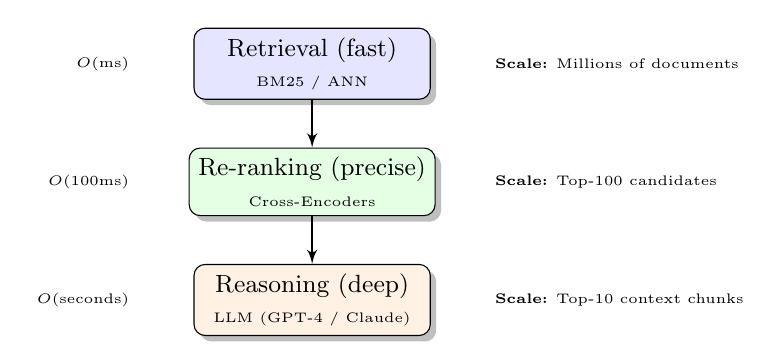
\begin{tikzpicture}[
    node distance=0.8cm,
    label/.style={font=\tiny, gray},
    vstep/.style={rectangle, draw, rounded corners, minimum width=3cm, minimum height=0.8cm, align=center, font=\small, drop shadow}
]
    \node[vstep, fill=blue!10] (ret) at (0, 3) {Retrieval (fast) \\ \tiny BM25 / ANN};
    \node[vstep, fill=green!10] (rank) at (0, 1.5) {Re-ranking (precise) \\ \tiny Cross-Encoders};
    \node[vstep, fill=orange!10] (llm) at (0, 0) {Reasoning (deep) \\ \tiny LLM (GPT-4 / Claude)};
    
    \draw[->, thick, >=latex'] (ret) -- (rank);
    \draw[->, thick, >=latex'] (rank) -- (llm);
    
    \node[anchor=west] at (2.2, 3) {\tiny \textbf{Scale:} Millions of documents};
    \node[anchor=west] at (2.2, 1.5) {\tiny \textbf{Scale:} Top-100 candidates};
    \node[anchor=west] at (2.2, 0) {\tiny \textbf{Scale:} Top-10 context chunks};
    
    \node[anchor=east] at (-2.2, 3) {\tiny $O(\text{ms})$};
    \node[anchor=east] at (-2.2, 1.5) {\tiny $O(100\text{ms})$};
    \node[anchor=east] at (-2.2, 0) {\tiny $O(\text{seconds})$};
\end{tikzpicture}

\end{center}

\begin{keytakeaway}
\textbf{Indexing sets the ceiling.} Re-ranking and LLM reasoning can only refine what retrieval finds. A missed document is lost forever.
\end{keytakeaway}

\subsection{Production Checklist}

\begin{multicols}{2}
\textbf{Sparse Index:}
\begin{itemize}[label=$\square$,nosep]
    \item Compression enabled
    \item Stop words handled
    \item Stemming appropriate
    \item Field boosting configured
    \item Metadata filterable
\end{itemize}

\textbf{Dense Index (IVF+PQ):}
\begin{itemize}[label=$\square$,nosep]
    \item Vectors normalized
    \item $n_{\mathrm{probe}}$ tuned
    \item Memory budget met
    \item PQ training data representative
\end{itemize}

\columnbreak

\textbf{Monitoring:}
\begin{itemize}[label=$\square$,nosep]
    \item Track recall@$k$ vs.\ exact search
    \item Monitor p95/p99 latency
    \item Alert on index growth
    \item Log query/document drift
\end{itemize}
\end{multicols}

%=======================================================================
\section{Summary and Next Steps}
\label{sec:summary}
%=======================================================================

\subsection{What We Covered}

\begin{enumerate}
    \item \textbf{Sparse Indexing:} Inverted index structure, text preprocessing, compression (gap + VB encoding), PyTerrier demo.
    \item \textbf{Dense Indexing:} ANN search, IVF+PQ (clustering + compression), FAISS demo.
    \item \textbf{Design Decisions:} When to use sparse vs.\ dense vs.\ hybrid; scaling; pitfalls.
\end{enumerate}

\subsection{Key Takeaways}

\begin{enumerate}
    \item \textbf{Inverted indexes are the backbone.} BM25 remains highly competitive for exact/entity queries.
    \item \textbf{Dense retrieval enables semantic search,} but requires ANN techniques (IVF+PQ) at scale.
    \item \textbf{Candidate generation is the bottleneck.} Indexing determines what re-rankers/LLMs can see.
    \item \textbf{Scalability requires compression.} PQ is vital for fitting large indexes in memory.
\end{enumerate}

\subsection{Connection to Upcoming Lectures}

\begin{itemize}[nosep]
    \item \textbf{Lecture 3 (Ranking):} BM25 uses inverted indexes; query expansion operates on sparse retrieval.
    \item \textbf{Lecture 4 (Transformer Re-rankers):} Re-rank candidates from today's retrieval stage.
    \item \textbf{Lecture 5 (Dense Retrieval Deep Dive):} Bi-encoders, training; ANN indexing is prerequisite.
    \item \textbf{Lecture 6 (Learning to Rank):} Combine sparse + dense scores; learn fusion weights.
\end{itemize}

%=======================================================================
% REFERENCES
%=======================================================================
\begin{thebibliography}{99}

\bibitem{lewis2020rag}
P.~Lewis, E.~Perez, A.~Piktus, F.~Petroni, V.~Karpukhin, N.~Goyal, H.~K\"uttler, M.~Lewis, W.~Yih, T.~Rockt\"aschel, S.~Riedel, and D.~Kiela.
Retrieval-augmented generation for knowledge-intensive NLP tasks.
\emph{NeurIPS}, 2020.

\bibitem{salton1975vector}
G.~Salton, A.~Wong, and C.~S.~Yang.
A vector space model for automatic indexing.
\emph{Communications of the ACM}, 18(11):613--620, 1975.

\bibitem{porter1980algorithm}
M.~F.~Porter.
An algorithm for suffix stripping.
\emph{Program}, 14(3):130--137, 1980.

\bibitem{reimers2019sentence}
N.~Reimers and I.~Gurevych.
Sentence-BERT: Sentence embeddings using Siamese BERT-networks.
\emph{EMNLP-IJCNLP}, pages 3982--3992, 2019.

\bibitem{indyk1998approximate}
P.~Indyk and R.~Motwani.
Approximate nearest neighbors: Towards removing the curse of dimensionality.
\emph{STOC}, pages 604--613, 1998.

\bibitem{jegou2011product}
H.~J\'egou, M.~Douze, and C.~Schmid.
Product quantization for nearest neighbor search.
\emph{IEEE TPAMI}, 33(1):117--128, 2011.

\bibitem{johnson2019billion}
J.~Johnson, M.~Douze, and H.~J\'egou.
Billion-scale similarity search with GPUs.
\emph{IEEE Transactions on Big Data}, 7(3):535--547, 2021.

\bibitem{malkov2018efficient}
Y.~A.~Malkov and D.~A.~Yashunin.
Efficient and robust approximate nearest neighbor search using Hierarchical Navigable Small World graphs.
\emph{IEEE TPAMI}, 42(4):824--836, 2020.

\bibitem{lin2021deepimpact}
J.~Lin et al.
A few brief notes on DeepImpact, COIL, and a conceptual framework for information retrieval techniques.
\emph{arXiv:2106.14807}, 2021.

\bibitem{macdonald2021pyterrier}
C.~Macdonald, N.~Tonellotto, S.~MacAvaney, and I.~Ounis.
PyTerrier: Declarative experimentation in Python from BM25 to dense retrieval.
\emph{CIKM}, pages 4526--4533, 2021.

\bibitem{manning2008introduction}
C.~D.~Manning, P.~Raghavan, and H.~Sch\"utze.
\emph{Introduction to Information Retrieval}.
Cambridge University Press, 2008.
\url{https://nlp.stanford.edu/IR-book/}

\bibitem{robertson2009bm25}
S.~Robertson and H.~Zaragoza.
The probabilistic relevance framework: BM25 and beyond.
\emph{Foundations and Trends in IR}, 3(4):333--389, 2009.

\end{thebibliography}

\end{document}